\documentclass[11pt]{article}
\usepackage{amsmath,amssymb,amsthm}
\usepackage{geometry}
\usepackage{booktabs}
\usepackage{graphicx}
\usepackage{hyperref}
\usepackage{enumitem}
\usepackage{listings}
\usepackage{xcolor}
\usepackage{longtable}
\usepackage{array}

\geometry{letterpaper, margin=1in}

\lstset{
  basicstyle=\ttfamily\small,
  keywordstyle=\color{blue},
  commentstyle=\color{gray},
  stringstyle=\color{red},
  breaklines=true,
  columns=fullflexible,
  keepspaces=true,
  language=C++
}

\title{\textbf{Formation Engine Methodology} \\
\Large Section KF --- Kinetic Formation, Organic Ontology, \\
and the Thermodynamic--Kinetic Distinction}
\author{Formation Engine Development Team}
\date{Version 4.0.0 --- April 2026}

\begin{document}
\maketitle
\tableofcontents

% ═══════════════════════════════════════════════════════════════════════════
\section{Introduction: What This Section Adds}
\label{sec:intro}
% ═══════════════════════════════════════════════════════════════════════════

Previous sections documented:

\begin{itemize}[leftmargin=2em]
  \item \S6 --- formation physics (VSEPR prediction, MD evolution, FIRE quench, scoring)
  \item \S8--9 --- reaction prediction (Fukui, HSAB, Bell--Evans--Polanyi)
  \item \S8b --- heat-gated template control (the 3-digit $h$ scalar)
\end{itemize}

This section introduces three additions that deepen the formation engine
without breaking existing architecture:

\begin{enumerate}[leftmargin=2em]
  \item \textbf{Kinetic formation scoring.}
        The distinction between \emph{most stable product} and
        \emph{most likely to actually form} becomes a first-class concept.
  \item \textbf{Organic ontology layer.}
        A separate classification system for organic candidates, carrying
        chemistry-aware descriptors beyond what lattice-based categories provide.
  \item \textbf{Universal kinetic engine.}
        One engine, many domain adapters.  Not separate kinetic engines for
        organics, metals, droplets, crystals, beams, decay, and salts.
\end{enumerate}

\textbf{Implementation:}
\begin{itemize}[leftmargin=2em]
  \item \texttt{atomistic/kinetic/formation\_kinetics.hpp}
  \item \texttt{atomistic/classify/organic\_candidate.hpp}
\end{itemize}

\textbf{Compatibility:} integrates with the existing \texttt{ReactionEngine}
(topology rewrites and Fukui scoring), \texttt{HeatGateController} (\S8b),
\texttt{GibbsCalculator} (thermodynamics.hpp), and
\texttt{MaterialCase} / \texttt{TechnicalReport} (report\_engine.hpp).

% ═══════════════════════════════════════════════════════════════════════════
\section{The Central Distinction: Thermodynamic vs.\ Kinetic Product}
\label{sec:distinction}
% ═══════════════════════════════════════════════════════════════════════════

For any system---organic, inorganic, or mixed---two questions are
fundamentally different:

\begin{center}
\begin{tabular}{lp{8cm}}
\toprule
Question & Meaning \\
\midrule
\textbf{What is most stable?} &
  Lowest long-term free energy.
  The thermodynamic product.
  Reached given infinite equilibration time. \\
\textbf{What actually forms?} &
  Lowest effective barrier pathway.
  The kinetic product.
  Observed at finite reaction time. \\
\bottomrule
\end{tabular}
\end{center}

The engine must compute \emph{both} rankings and present them as
first-class outputs.  The expected output format is:

\begin{center}
\begin{tabular}{lccl}
\toprule
Candidate & Thermo Rank & Kinetic Rank & Expected Observation \\
\midrule
A & 1 & 3 & likely after long equilibration \\
B & 2 & 1 & likely early product \\
C & 3 & 2 & transient intermediate \\
\bottomrule
\end{tabular}
\end{center}

\textbf{Implementation:} \texttt{FormationScore} and \texttt{CandidateRow}
in \texttt{formation\_kinetics.hpp}.

% ═══════════════════════════════════════════════════════════════════════════
\section{Formation Likelihood: The Full Scoring Function}
\label{sec:scoring}
% ═══════════════════════════════════════════════════════════════════════════

The probability that product $i$ is observed is modelled as:

\begin{equation}
\label{eq:formation_prob}
P(\text{product}\; i) \;\sim\;
f\!\left(E_i,\;\Delta G_i,\;E_{a,i},\;\tau,\;T,\;
\text{solvent},\;\text{crowding},\;\text{path accessibility}\right)
\end{equation}

This decomposes into four scoring branches.

\subsection{Thermodynamic Branch ($S_\text{thermo}$)}

Based on the final static energy and Gibbs free energy of formation:

\begin{equation}
S_\text{thermo} = \sigma\!\left(\frac{-\Delta G_i}{kT}\right)
\end{equation}

where $\sigma$ is a sigmoid mapping $(-\infty,+\infty) \to [0,1]$.

\subsection{Kinetic Branch ($S_\text{kinetic}$)}

\begin{equation}
\label{eq:skinetic}
S_\text{kinetic} = w_1 A_\text{path}
                 + w_2 R_\text{encounter}
                 + w_3 S_\text{steric}
                 + w_4 T_\text{window}
                 + w_5 E_\text{barrier}
\end{equation}

\begin{center}
\begin{tabular}{lll}
\toprule
Component & Symbol & Meaning \\
\midrule
Pathway accessibility     & $A_\text{path}$      & Is a viable reaction pathway geometrically open? \\
Encounter likelihood      & $R_\text{encounter}$  & Do reactants meet at sufficient rate? \\
Steric permissibility     & $S_\text{steric}$     & Is the transition sterically allowed? \\
Temperature suitability   & $T_\text{window}$     & Is the system in the right thermal window? \\
Barrier penalty           & $E_\text{barrier}$    & How high is the activation barrier? \\
\bottomrule
\end{tabular}
\end{center}

Default weights: $w_1{=}0.20$, $w_2{=}0.20$, $w_3{=}0.20$,
$w_4{=}0.15$, $w_5{=}0.25$.

\textbf{Implementation:} \texttt{KineticWeights} struct,
\texttt{FormationScore} fields \texttt{A\_path} through
\texttt{E\_barrier\_penalty}.

\subsection{Environmental Branch ($S_\text{env}$)}

\begin{equation}
S_\text{env} = \tfrac{1}{2}\left(S_\text{solvent} + S_\text{crowding}\right)
\end{equation}

Solvent stabilisation and steric crowding from the local environment,
evaluated per-event by the \texttt{DomainAdapter::compute\_environment()}
callback.

\subsection{Data Branch ($S_\text{data}$)}

Incorporates meta-scores from the existing HGST and V4 scoring system
($\gamma$, $Q_\text{data}$, $C_\text{compact}$).

\subsection{Combined Formation Score}

\begin{equation}
\label{eq:sform}
S_\text{form} = \alpha\, S_\text{thermo}
              + \beta\, S_\text{kinetic}
              + \chi\, S_\text{env}
              + \delta\, S_\text{data}
\end{equation}

Defaults: $\alpha{=}0.30$, $\beta{=}0.35$, $\chi{=}0.20$, $\delta{=}0.15$.

\textbf{Implementation:} \texttt{FormationKineticsEngine::score\_candidate()},
\texttt{FormationKineticsEngine::rank\_candidates()}.

% ═══════════════════════════════════════════════════════════════════════════
\section{Universal Kinetic Engine Architecture}
\label{sec:universal}
% ═══════════════════════════════════════════════════════════════════════════

\subsection{Why One Engine, Not Many}

A separate kinetic engine for each domain (organics, metals, droplets,
crystal growth, beam transport, decay, salt chemistry) would be a
maintenance graveyard with extra folders.

At the highest level, kinetics is always:

\begin{quote}
State at time $t$ $\;\to\;$ possible transitions $\;\to\;$
rates/probabilities $\;\to\;$ new state
\end{quote}

The actual abstraction:

\begin{equation}
\label{eq:kinetic_tuple}
\mathcal{K} = \{\,\mathcal{S},\; \mathcal{E},\; \mathcal{R},\; \mathcal{U}\,\}
\end{equation}

\begin{center}
\begin{tabular}{lp{9cm}}
\toprule
Symbol & Meaning \\
\midrule
$\mathcal{S}$ & State space: what exists right now \\
$\mathcal{E}$ & Event space: what \textsc{can} happen \\
$\mathcal{R}$ & Rate laws: how fast each event occurs \\
$\mathcal{U}$ & Update rules: how the state changes after an event \\
\bottomrule
\end{tabular}
\end{center}

\subsection{What Changes by Domain}

The engine is universal.  The meaning of \emph{state} and \emph{barrier}
changes.

\begin{center}
\begin{tabular}{lp{4cm}p{4cm}p{4cm}}
\toprule
Domain & State & Events & Barrier means \\
\midrule
Organics &
  connectivity, conformer, medium, reactive site map &
  substitution, elimination, cyclisation, rearrangement, decomposition &
  orbital mismatch, steric hindrance, charge separation cost, torsional preorganisation \\[6pt]
Crystal growth &
  lattice seed, coordination, defects, surface, temperature field &
  attachment, vacancy migration, dislocation, recrystallisation, defect annihilation &
  attachment penalty, diffusion activation, strain energy, surface energy mismatch \\[6pt]
Droplet / beam &
  radius, temperature, velocity, oxidation, surface tension, gas density &
  flight, collision, evaporation, coalescence, impact, freezing &
  impact threshold, wetting threshold, thermal loss, contamination \\[6pt]
Decay-aware material &
  isotope identity, decay age, coordination, daughter history, damage tally &
  $\alpha$/$\beta$/$\gamma$ emission, transmutation, lattice disruption, He accumulation &
  NOT just chemical barrier: hazard / deterministic emission law, damage propagation threshold \\
\bottomrule
\end{tabular}
\end{center}

\textbf{Implementation:} \texttt{DomainAdapter} pure virtual base class.
Each domain provides \texttt{enumerate\_transitions()},
\texttt{rate\_law\_for()}, \texttt{apply\_event()},
\texttt{compute\_environment()}, \texttt{history\_score()}.

\subsection{Event Types}

The \texttt{EventType} enumeration covers all domains without domain-specific
subclassing.  For events where the emission particle does not yet exist in the
model (e.g.\ an alpha particle in a decay chain where the daughter nuclide has
not been coded), the adapter \textbf{must} record the event and leave a
placeholder.  Silent data invention is forbidden.

\textbf{Full list in} \texttt{formation\_kinetics.hpp}, lines covering
\texttt{BOND\_FORMATION} through \texttt{HELIUM\_ACCUMULATION}.

\subsection{Rate Laws}

\begin{center}
\begin{tabular}{llp{6.5cm}}
\toprule
Type & Formula & Use \\
\midrule
\texttt{ARRHENIUS}         & $k = A\,e^{-E_a/k_BT}$
  & Chemical bond events, thermal processes \\
\texttt{HAZARD}            & $\lambda = \ln 2 / t_{1/2}$
  & Nuclear decay (temperature-independent) \\
\texttt{COLLISION\_THEORY} & $k = \sigma\, v_\text{rel}\, n$
  & Gas-phase encounters, beam collisions \\
\texttt{BARRIERLESS}       & $k = A$ (pre-exponential only)
  & Diffusion-limited reactions \\
\texttt{DETERMINISTIC\_STEP} & fires at fixed $\Delta t$
  & MD-like stepping \\
\texttt{CUSTOM}            & $\lambda$ from adapter
  & Domain-specific extensions \\
\bottomrule
\end{tabular}
\end{center}

% ═══════════════════════════════════════════════════════════════════════════
\section{Organic Ontology: A Separate Classification Layer}
\label{sec:organic}
% ═══════════════════════════════════════════════════════════════════════════

\subsection{Why Organics Need Their Own Layer}

The existing inorganic classification categories (\texttt{ElementCategory}
in \texttt{comprehensive\_elements.hpp}: noble metal, transition metal,
alkali, actinide, halogen, etc.)\ are useful for materials-first logic.

For organics, these categories carry almost no information about chemical
behaviour.  Carbon is always \texttt{NONMETAL}, but the difference between
an alkane and a nitrile is enormous.

\subsection{Organic Family Tags}

\begin{center}
\begin{longtable}{lp{8.5cm}}
\toprule
Family & Determines \\
\midrule
\endhead
\texttt{ALKANE}               & saturated, low polarity, flexible chain \\
\texttt{ALKENE}               & unsaturated, electrophilic addition sites \\
\texttt{ALKYNE}               & linear geometry, strong triple bond \\
\texttt{AROMATIC}             & rigid ring, delocalised $\pi$, electrophilic substitution \\
\texttt{HETEROAROMATIC}       & aromatic with N/O/S, altered reactivity \\
\texttt{ALCOHOL}              & OH donor, H-bond rich \\
\texttt{ETHER}                & acceptor-only, low reactivity \\
\texttt{KETONE}               & carbonyl, nucleophilic addition site \\
\texttt{ALDEHYDE}             & terminal carbonyl, more reactive than ketone \\
\texttt{CARBOXYLIC\_ACID}     & acidic proton, H-bond donor+acceptor \\
\texttt{ESTER}                & hydrolysis-prone, moderate polarity \\
\texttt{AMIDE}                & resonance-stabilised, strong H-bond \\
\texttt{AMINE}                & basic, nucleophilic, H-bond donor \\
\texttt{NITRILE}              & linear, polarised triple bond \\
\texttt{HALOGENATED\_ORGANIC} & leaving group, dipole, substitution-prone \\
\texttt{ORGANOMETALLIC}       & metal--carbon bond, catalytic relevance \\
\texttt{POLYMER\_PRECURSOR}   & polymerisable double bond or functional group \\
\texttt{CROSSLINKABLE}        & multi-functional, network-forming \\
\texttt{RADICAL\_PRONE}       & weak bonds, radical chain initiation \\
\texttt{CONJUGATED}           & extended $\pi$, optical/electronic properties \\
\texttt{RIGID\_RING}          & limited conformational freedom \\
\texttt{FLEXIBLE\_CHAIN}      & many torsional DOF \\
\texttt{DONOR\_RICH}          & electron-rich, nucleophilic character \\
\texttt{ACCEPTOR\_RICH}       & electron-poor, electrophilic character \\
\bottomrule
\end{longtable}
\end{center}

\textbf{Implementation:} \texttt{OrganicFamily} enum in
\texttt{organic\_candidate.hpp}.

\subsection{The Organic Identity Card}

Beyond lattice parameters and cohesive energy, the organic candidate object
carries:

\begin{center}
\begin{tabular}{lp{7cm}}
\toprule
Descriptor block & Contents \\
\midrule
Connectivity     & formula, functional groups, ring count, aromatic count \\
Topology         & sp3/sp2/sp counts, rotatable bonds, chiral centres \\
Chemistry scores & steric, polarity, H-bond donor/acceptor, conjugation, strain \\
Formation scores & thermo, kinetic, packing, decomposition risk, $S_\text{form}$ \\
Reactive site map & per-atom Fukui indices, local softness, site type labels \\
Donor/acceptor map & per-atom H-bond donor/acceptor classification \\
Polarity map     & per-atom partial charges and polarity contributions \\
Torsion profiles & per-rotatable-bond barrier heights and symmetry folds \\
\bottomrule
\end{tabular}
\end{center}

\textbf{Implementation:}
\texttt{OrganicCandidate} struct with nested \texttt{ReactiveSite},
\texttt{DonorAcceptor}, \texttt{PolaritySite}, \texttt{TorsionProfile}
records.  \texttt{OrganicClassifier} derives all fields from
\texttt{atomistic::State}.

% ═══════════════════════════════════════════════════════════════════════════
\section{Integration with Existing Systems}
\label{sec:integration}
% ═══════════════════════════════════════════════════════════════════════════

\subsection{Reaction Engine (\S8--9)}

The existing \texttt{ReactionEngine} handles:
\begin{itemize}[leftmargin=2em]
  \item Fukui function computation
  \item HSAB site matching
  \item Bell--Evans--Polanyi barrier estimation
  \item Topology rewriting (bond break / form)
\end{itemize}

The kinetic formation engine sits one layer above:
it decides \emph{which} transitions are attempted, \emph{at what rate},
and tracks time evolution.  The reaction engine remains the workhorse for
topology changes; the kinetic engine selects and sequences them.

\subsection{Heat-Gated Control (\S8b)}

The heat parameter $h \in \{0,\ldots,999\}$ controls which
bio-templates are active.  The kinetic engine inherits this gating:
events requiring inactive templates are excluded from the transition
enumeration step.

\subsection{Gibbs Calculator}

The \texttt{GibbsCalculator} in \texttt{thermodynamics.hpp} provides
$\Delta G$ values used directly by
\texttt{FormationScore::delta\_G\_eV}
and the thermodynamic branch scoring.

\subsection{HGST Matrix}

The 5D state vector $[\rho_D, \Gamma, S, \Pi, Q]$ feeds the
data branch of the formation score via the existing
\texttt{hgst::BondScorer} and \texttt{hgst::StateVector}.

\subsection{Report Engine}

\texttt{MaterialCase} and \texttt{TechnicalReport} gain a new optional
field path: the kinetic ranking table can be included in reports
alongside existing experiment results.

\subsection{Visualization}

The crystal card popup (\texttt{crystal\_card\_popup.py}) already exports
JSON snapshots with $\gamma$, $Q_\text{data}$, $C_\text{compact}$.
Future snapshots will include \texttt{thermo\_rank},
\texttt{kinetic\_rank}, and \texttt{S\_form} from the kinetic engine.

The \texttt{atoms\_vs\_bonds.png} figure
(Figure~\ref{fig:atoms_vs_bonds}) illustrates the scaling relationship
between atom count and bond count that underpins the transition
enumeration: more bonds means more possible topology-change events.

\begin{figure}[h]
\centering
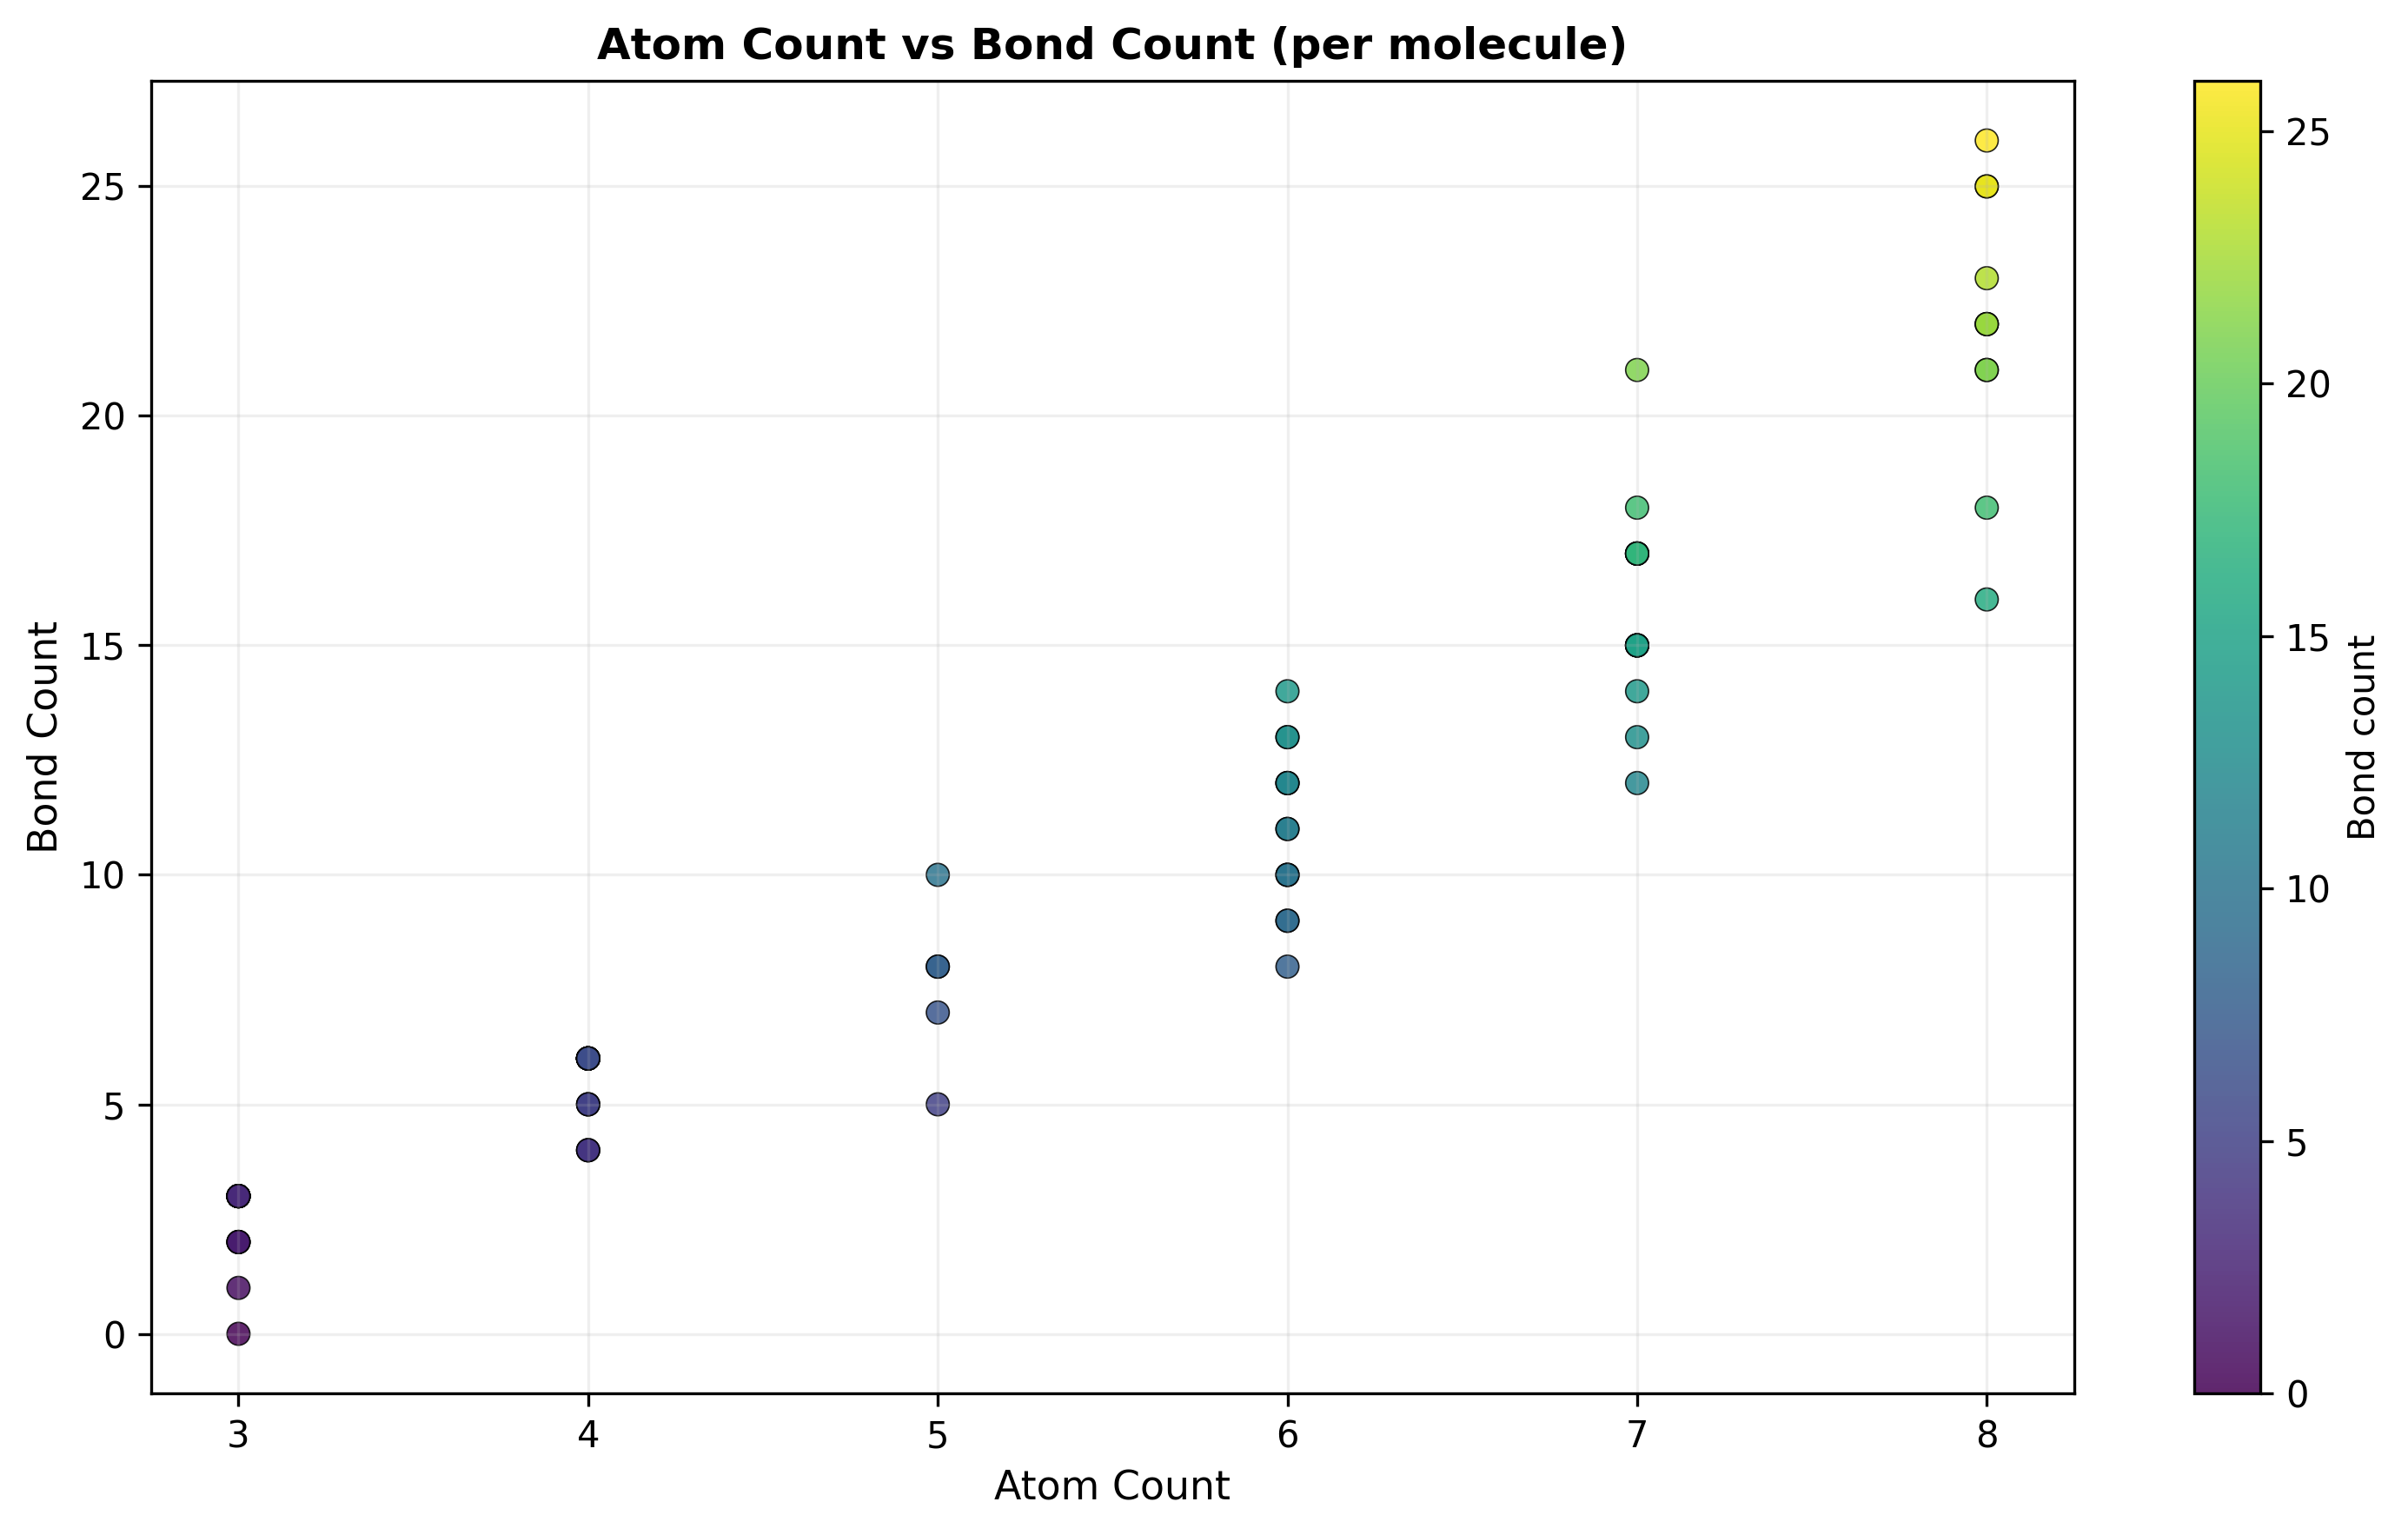
\includegraphics[width=0.6\textwidth]{figures/atoms_vs_bonds.png}
\caption{Atom count vs.\ bond count for representative structures.
The bond count determines the upper bound on topology-change transitions
enumerated per kinetic step.}
\label{fig:atoms_vs_bonds}
\end{figure}

% ═══════════════════════════════════════════════════════════════════════════
\section{Engine Lifecycle: Step-by-Step}
\label{sec:lifecycle}
% ═══════════════════════════════════════════════════════════════════════════

A single kinetic step proceeds as:

\begin{enumerate}[leftmargin=2em]
  \item \textbf{Enumerate.}
        \texttt{DomainAdapter::enumerate\_transitions(state)} produces
        all transitions from the current state.
  \item \textbf{Rate.}
        For each transition, the adapter provides a \texttt{RateLaw};
        the engine evaluates $k_i = f(\text{state}, \text{env}, E_a, T)$.
  \item \textbf{Score.}
        The engine computes all four branches
        ($S_\text{thermo}$, $S_\text{kinetic}$, $S_\text{env}$,
        $S_\text{data}$) and combines them into $S_\text{form}$.
  \item \textbf{Select.}
        Rate-weighted stochastic selection (Gillespie-like) picks
        the next event.
  \item \textbf{Apply.}
        \texttt{DomainAdapter::apply\_event(state, event)} updates
        the state.  Time advances by $\Delta t = -\ln(u) / \sum k_i$.
  \item \textbf{Record.}
        The event is appended to the trail; lineage hash is updated.
\end{enumerate}

Multi-step evolution runs steps 1--6 in a loop until
\texttt{max\_events} or \texttt{max\_time} is reached.

% ═══════════════════════════════════════════════════════════════════════════
\section{Domain Adapter Examples}
\label{sec:adapters}
% ═══════════════════════════════════════════════════════════════════════════

\subsection{Organics}

\begin{center}
\begin{tabular}{ll}
\toprule
Adapter callback & Returns \\
\midrule
\texttt{enumerate\_transitions} &
  substitution, elimination, cyclisation, rearrangement, decomposition \\
\texttt{rate\_law\_for} &
  Arrhenius with BEP-estimated barriers \\
\texttt{apply\_event} &
  topology rewrite via \texttt{ReactionEngine} \\
\texttt{compute\_environment} &
  solvent dielectric screening, crowding from \texttt{steric\_score} \\
\texttt{history\_score} &
  formation path memory (radical chain propagation) \\
\bottomrule
\end{tabular}
\end{center}

\subsection{Crystal Growth}

\begin{center}
\begin{tabular}{ll}
\toprule
Adapter callback & Returns \\
\midrule
\texttt{enumerate\_transitions} &
  attachment, vacancy migration, dislocation, recrystallisation \\
\texttt{rate\_law\_for} &
  Arrhenius (diffusion barrier) or barrierless (adsorption) \\
\texttt{apply\_event} &
  lattice topology update (add/remove atom, move defect) \\
\texttt{compute\_environment} &
  local temperature gradient, surface energy anisotropy \\
\texttt{history\_score} &
  defect accumulation penalty \\
\bottomrule
\end{tabular}
\end{center}

\subsection{Droplet / Beam Transport}

\begin{center}
\begin{tabular}{ll}
\toprule
Adapter callback & Returns \\
\midrule
\texttt{enumerate\_transitions} &
  flight, collision, evaporation, coalescence, impact, freezing \\
\texttt{rate\_law\_for} &
  collision theory ($k = \sigma\, v_\text{rel}\, n$) \\
\texttt{apply\_event} &
  update radius, velocity, temperature, oxidation \\
\texttt{compute\_environment} &
  local gas density, substrate proximity \\
\texttt{history\_score} &
  prior collision chain (splashing history) \\
\bottomrule
\end{tabular}
\end{center}

\subsection{Decay-Aware Material}

\begin{center}
\begin{tabular}{ll}
\toprule
Adapter callback & Returns \\
\midrule
\texttt{enumerate\_transitions} &
  $\alpha$/$\beta$/$\gamma$ emission, transmutation, He accumulation \\
\texttt{rate\_law\_for} &
  Hazard: $\lambda = \ln 2 / t_{1/2}$ \\
\texttt{apply\_event} &
  isotope transmutation, lattice disruption recording.
  If emission particle does not exist in model,
  record event and await context. \\
\texttt{compute\_environment} &
  radiation damage tally, daughter product neighbourhood \\
\texttt{history\_score} &
  cumulative damage penalty, prior transmutation chain \\
\bottomrule
\end{tabular}
\end{center}

% ═══════════════════════════════════════════════════════════════════════════
\section{Static Structure as Special Case}
\label{sec:static}
% ═══════════════════════════════════════════════════════════════════════════

A ``final observed structure'' is one of three things:

\begin{enumerate}[leftmargin=2em]
  \item \textbf{Lowest static energy} --- the thermodynamic product.
        The result of FIRE quench to a local minimum on the PES\@.
  \item \textbf{Sample-specific end energy} --- the kinetic product.
        The state reached after a finite number of kinetic events at a
        given temperature.
  \item \textbf{Energy at random time frame} --- a snapshot of the
        time-evolving system, not necessarily at equilibrium.
\end{enumerate}

The kinetic engine naturally handles all three:
case~1 is \texttt{evolve()} with infinite time and zero temperature;
case~2 is \texttt{evolve()} with finite \texttt{max\_time};
case~3 is a single call to \texttt{step()} at an arbitrary point in the
trajectory.

% ═══════════════════════════════════════════════════════════════════════════
\section{File Manifest}
\label{sec:files}
% ═══════════════════════════════════════════════════════════════════════════

\begin{center}
\begin{tabular}{lp{7.5cm}}
\toprule
File & Purpose \\
\midrule
\texttt{atomistic/kinetic/formation\_kinetics.hpp} &
  Universal kinetic engine: \texttt{KineticState},
  \texttt{TransitionEvent}, \texttt{EventType},
  \texttt{RateLaw}, \texttt{FormationScore},
  \texttt{KineticWeights}, \texttt{CandidateRow},
  \texttt{DomainAdapter}, \texttt{FormationKineticsEngine} \\
\texttt{atomistic/classify/organic\_candidate.hpp} &
  Organic ontology: \texttt{OrganicFamily},
  \texttt{OrganicCandidate} (with nested site maps),
  \texttt{OrganicClassifier} \\
\texttt{atomistic/reaction/engine.hpp} &
  Existing reaction engine (unchanged, consumed by kinetic layer) \\
\texttt{atomistic/reaction/causal.hpp} &
  Causal discovery engine (unchanged, feeds history scoring) \\
\texttt{atomistic/reaction/heat\_gate.hpp} &
  Heat-gated template control (unchanged) \\
\texttt{include/thermo/thermodynamics.hpp} &
  Gibbs calculator (unchanged, consumed for $\Delta G$) \\
\texttt{include/hgst/hgst\_matrix.hpp} &
  HGST scoring (unchanged, feeds data branch) \\
\texttt{include/core/report\_engine.hpp} &
  Report engine (unchanged, receives ranking table) \\
\texttt{docs/figures/atoms\_vs\_bonds.png} &
  Scaling figure referenced in \S\ref{sec:integration} \\
\bottomrule
\end{tabular}
\end{center}

% ═══════════════════════════════════════════════════════════════════════════
\section{Design Constraints}
\label{sec:constraints}
% ═══════════════════════════════════════════════════════════════════════════

\begin{enumerate}[leftmargin=2em]
  \item No data is hardcoded as a Z array.
        All descriptors are derived from the connectivity graph and
        element properties at runtime.
  \item Terminology: use \emph{atomistic} throughout.
        The word \emph{meso} is forbidden.
  \item If an emission particle does not yet exist in the model
        (e.g.\ alpha particle, positron), the adapter records the event
        and leaves a placeholder.  It does not silently invent data.
  \item Anti-black-box: every rate, every barrier, every event selection
        decision is inspectable and deterministic given seed.
  \item The universal engine is ONE engine with domain adapters,
        not separate engines per domain.
\end{enumerate}

\vspace{2em}
\hrule
\vspace{0.5em}
{\small\itshape
VSEPR-SIM Formation Engine Methodology ---
Section KF: Kinetic Formation ---
Version 4.0.0, April 2026.}

\end{document}
